% Based on Stereographic and cylindrical map projections
% Author: Tomasz M. Trzeciak
% Source: LaTeX-Community.org 
%         <http://www.latex-community.org/viewtopic.php?f=4&t=2111>

\usetikzlibrary{calc,fadings,decorations.pathreplacing,decorations}
%% helper macros

\newcommand\pgfmathsinandcos[3]{%
  \pgfmathsetmacro#1{sin(#3)}%
  \pgfmathsetmacro#2{cos(#3)}%
}
\newcommand\LongitudePlane[3][current plane]{%
  \pgfmathsinandcos\sinEl\cosEl{#2} % elevation
  \pgfmathsinandcos\sint\cost{#3} % azimuth
  \tikzset{#1/.style={cm={\cost,\sint*\sinEl,0,\cosEl,(0,0)}}}
}
\newcommand\LatitudePlane[3][current plane]{%
  \pgfmathsinandcos\sinEl\cosEl{#2} % elevation
  \pgfmathsinandcos\sint\cost{#3} % latitude
  \pgfmathsetmacro\yshift{\cosEl*\sint}
  \tikzset{#1/.style={cm={\cost,0,0,\cost*\sinEl,(0,\yshift)}}} %
}
\newcommand\DrawLongitudeCircle[2][1]{
  \LongitudePlane{\angEl}{#2}
  \tikzset{current plane/.prefix style={scale=#1}}
   % angle of "visibility"
  \pgfmathsetmacro\angVis{atan(sin(#2)*cos(\angEl)/sin(\angEl))} %
  \draw[current plane] (\angVis:1) arc (\angVis:\angVis+180:1);
  \draw[current plane,dashed] (\angVis-180:1) arc (\angVis-180:\angVis:1);
}
\newcommand\DrawLatitudeCircle[2][1]{
  \LatitudePlane{\angEl}{#2}
  \tikzset{current plane/.prefix style={scale=#1}}
  \pgfmathsetmacro\sinVis{sin(#2)/cos(#2)*sin(\angEl)/cos(\angEl)}
  % angle of "visibility"
  \pgfmathsetmacro\angVis{asin(min(1,max(\sinVis,-1)))}
  \draw[current plane] (\angVis:1) arc (\angVis:-\angVis-180:1);
  \draw[current plane,dashed] (180-\angVis:1) arc (180-\angVis:\angVis:1);
}

%% document-wide tikz options and styles

\tikzset{%
  >=latex, % option for nice arrows
  inner sep=0pt,%
  outer sep=2pt,%
  mark coordinate/.style={inner sep=0pt,outer sep=0pt,minimum size=3pt,
    fill=black,circle}%
}

% \begin{tikzpicture} % "THE GLOBE" showcase

% \def\R{2.5} % sphere radius
% \def\angEl{35} % elevation angle
% \filldraw[ball color=white] (0,0) circle (\R);
% \foreach \t in {-80,-60,...,80} { \DrawLatitudeCircle[\R]{\t} }
% \foreach \t in {-5,-35,...,-175} { \DrawLongitudeCircle[\R]{\t} }

% \end{tikzpicture}

%%%%%%%%%%%%%%%%%%%%%%%%%%%%%%%%%%%%%%%%%%%%%%%%%%%%%%%%%%%%%%%%%%%%%%%%%%%%%%%%%%%%%

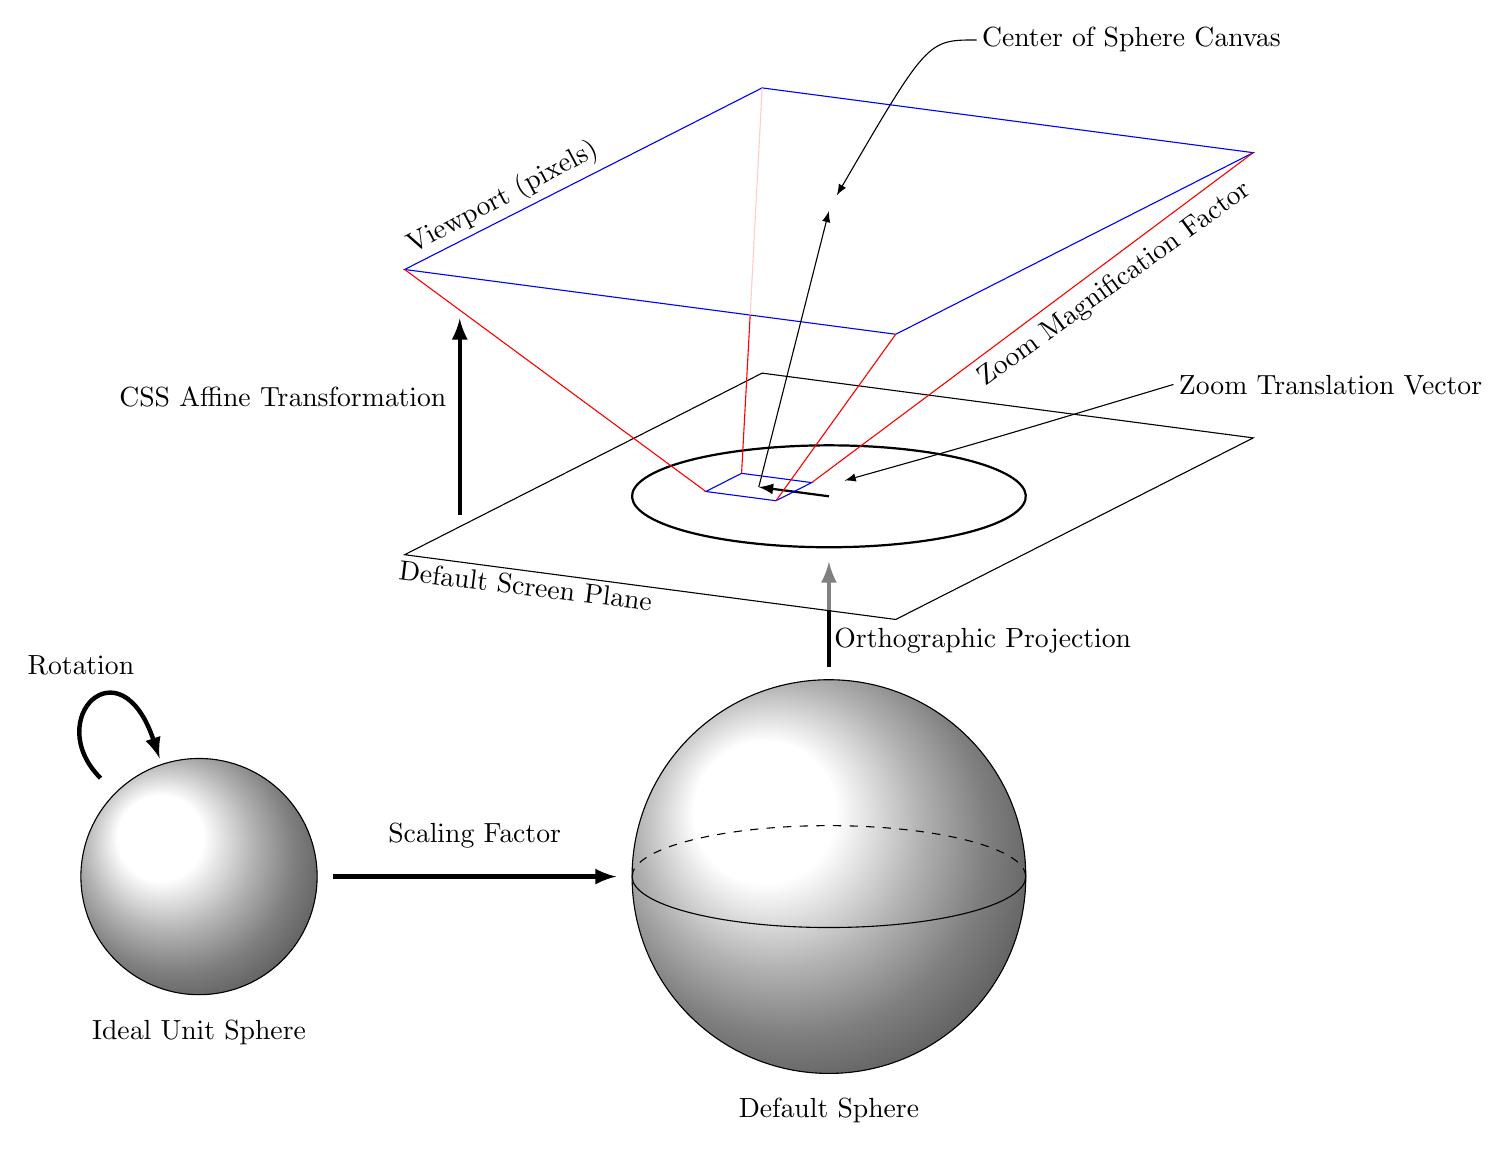
\begin{tikzpicture} % CENT

%% some definitions

\def\R{2.5} % sphere radius
\def\angEl{15} % elevation angle
\def\angAz{-117} % azimuth angle

%The coordinates of the rectangle zoom in the Viewport
\def\lcoord{-0.2*\R} 
\def\rcoord{0.2*\R}
\def\bcoord{-0.6*\R}
\def\fcoord{-0.2*\R}
\def\centerxcoord{-0.4*\R} %average of bcoord and fcoord
\def\centerycoord{0.0*\R} % average of lcoord and rcoord
%% working planes

\pgfmathsetmacro\H{\R*cos(\angEl)} % distance to north pole
\tikzset{DefaultScreenPlane/.style={cm={cos(\angAz),sin(\angAz)*sin(\angEl),-sin(\angAz),
                              cos(\angAz)*sin(\angEl),(0,2*\H)}}}
\tikzset{Viewport/.style={cm={cos(\angAz),sin(\angAz)*sin(\angEl),-sin(\angAz),
                              cos(\angAz)*sin(\angEl),(0,3.5*\H)}}}
\LongitudePlane[xzplane]{\angEl}{\angAz}
\LatitudePlane[equator]{\angEl}{0}

%% draw planes and sphere
\fill[ball color=white] (0,0) circle (\R); % 3D lighting effect
\draw (0,0) circle (\R);
\draw (0,-1.1*\R) node[below] {Default Sphere};

\fill[ball color=white] (-8,0) circle (0.6*\R); % 3D lighting effect
\draw (-8,0) circle (0.6*\R);
\draw (-8,-0.7*\R) node[below] {Ideal Unit Sphere};

\draw[ultra thick,->] (-6.3,0.0) -- (-2.7,0.0); 
\draw (-4.5,0.3) node[above]{Scaling Factor};

\draw (-9.5,2.5) node[above]{Rotation};
\draw[->, ultra thick] (-8,0)+(-0.5*\R,0.5*\R) .. controls (-10,2) and (-9,3) .. (-8.5,0.6*\R) ;

\draw[Viewport, color=blue] (-2*\R,-1.4*\R) rectangle (2.*\R,1.4*\R);
\draw[DefaultScreenPlane] (-2*\R,-1.4*\R) rectangle (2*\R,1.4*\R);

%$ Rectangle in the default screen plane
%Front Right corner
\path[DefaultScreenPlane] (\rcoord,\fcoord) coordinate (FRDSP);
%Front Left corner
\path[DefaultScreenPlane] (\lcoord,\fcoord) coordinate (FLDSP);
%Back Right corner
\path[DefaultScreenPlane] (\rcoord,\bcoord) coordinate (BRDSP);
%Back Left corner
\path[DefaultScreenPlane] (\lcoord,\bcoord) coordinate (BLDSP);
\path[DefaultScreenPlane] (\centerycoord,\centerxcoord) coordinate (center);
           
\path[DefaultScreenPlane] (0.5*\centerycoord,0.5*\centerxcoord) coordinate (midVector);
\path[DefaultScreenPlane] (0,0) coordinate (originDSP);

\path[DefaultScreenPlane] (2*\R,-1.4*\R) coordinate (FL);



%Front Right corner
\path[Viewport] (2*\R,1.4*\R) coordinate (FRSP);
%Front Left corner
\path[Viewport] (-2*\R,1.4*\R) coordinate (FLSP);
%Back Right corner
\path[Viewport] (2*\R,-1.4*\R) coordinate (BRSP);
%Back Left corner
\path[Viewport] (-2*\R,-1.4*\R) coordinate (BLSP);

\path[Viewport] (0,0) coordinate (origin);

\draw[ultra thick, ->] (FL)+(7mm,5mm) -- +(7mm,30mm);
\draw (FL)+(6mm,20mm) node[left] {CSS Affine Transformation};

\draw[<-] (origin)+(1mm,2mm) .. controls (0.5*\R,4.25*\R) .. (0.75*\R,4.25*\R) node[right]{Center of Sphere Canvas};
\draw[<-] (originDSP)+(2mm,2mm) .. controls (0.75*\R,2.2*\R) .. (1.75*\R,2.5*\R) node[right]{Zoom Translation Vector};

\path[Viewport] (2*\R,0.57*\R) coordinate (breakPoint);

\draw[color=red!20] (breakPoint) --  (BLSP);

\DrawLatitudeCircle[\R]{0} % equator





\draw[DefaultScreenPlane,->, thick] (0,0)  -- (center);
\draw[ultra thick] (0,1.1*\H) -- (0,1.4*\R);
\draw[->, ultra thick,color=gray] (0,1.4*\H) -- (0,1.6*\R);
\draw[DefaultScreenPlane, thick] (0,0) circle (\R);
\draw[DefaultScreenPlane,color=blue] (\rcoord,\fcoord) rectangle (\lcoord,\bcoord);
\draw[DefaultScreenPlane] (2*\R,-0.7*\R) node[below, rotate=-7] {Default Screen Plane};
\draw[thick] (0,1.2*\R) node[right] {Orthographic Projection};
\draw[color=red] (FRDSP) -- (FRSP);
\draw[color=red] (FLDSP) -- (FLSP);
\draw[color=red] (BRDSP) -- (BRSP);
\draw[color=red](BLDSP) -- (breakPoint);
\draw[->] (center) -- (origin);
\draw[Viewport] (0.8*\R,-1.4*\R) node[above, rotate=28] {Viewport (pixels)};
\draw[thick] (0.75*\R,2.5*\R) node[right, rotate=36 ] {Zoom Magnification Factor};

\end{tikzpicture}
%%%%%%%%%%%%%%%%%%%%%%%%%%%%%%%%%%%%%%%%%%%%%%%%%%%%%%%%%%%%%%%%%%%%%%%%%%%%%%%%%%%%%%
% \begin{tikzpicture} % MERC

% %% some definitions

% \def\R{3} % sphere radius
% \def\angEl{25} % elevation angle
% \def\angAz{-100} % azimuth angle
% \def\angPhiOne{-50} % longitude of point P
% \def\angPhiTwo{-35} % longitude of point Q
% \def\angBeta{33} % latitude of point P and Q

% %% working planes

% \pgfmathsetmacro\H{\R*cos(\angEl)} % distance to north pole
% \LongitudePlane[xzplane]{\angEl}{\angAz}
% \LongitudePlane[pzplane]{\angEl}{\angPhiOne}
% \LongitudePlane[qzplane]{\angEl}{\angPhiTwo}
% \LatitudePlane[equator]{\angEl}{0}

% %% draw background sphere

% \fill[ball color=white] (0,0) circle (\R); % 3D lighting effect
% %\fill[white] (0,0) circle (\R); % just a white circle
% \draw (0,0) circle (\R);

% %% characteristic points

% \coordinate (O) at (0,0);
% \coordinate[mark coordinate] (N) at (0,\H);
% \coordinate[mark coordinate] (S) at (0,-\H);
% \path[xzplane] (\R,0) coordinate (XE);
% \path[pzplane] (\angBeta:\R) coordinate (P);
% \path[pzplane] (\R,0) coordinate (PE);
% \path[qzplane] (\angBeta:\R) coordinate (Q);
% \path[qzplane] (\R,0) coordinate (QE);

% %% meridians and latitude circles

% % \DrawLongitudeCircle[\R]{\angAz} % xzplane
% % \DrawLongitudeCircle[\R]{\angAz+90} % yzplane
% \DrawLongitudeCircle[\R]{\angPhiOne} % pzplane
% \DrawLongitudeCircle[\R]{\angPhiTwo} % qzplane
% \DrawLatitudeCircle[\R]{\angBeta}
% \DrawLatitudeCircle[\R]{0} % equator

% % shifted equator in node with nested call to tikz 
% % (I didn't know it's possible)
% \node at (0,1.6*\R) { \tikz{\DrawLatitudeCircle[\R]{0}} };

% %% draw lines and put labels

% \draw (-\R,-\H) -- (-\R,2*\R) (\R,-\H) -- (\R,2*\R);
% \draw[->] (XE) -- +(0,2*\R) node[above] {$y$};
% \node[above=8pt] at (N) {$\mathbf{N}$};
% \node[below=8pt] at (S) {$\mathbf{S}$};
% \draw[->] (O) -- (P);
% \draw[dashed] (XE) -- (O) -- (PE);
% \draw[dashed] (O) -- (QE);
% \draw[pzplane,->,thin] (0:0.5*\R) to[bend right=15]
%     node[midway,right] {$\beta$} (\angBeta:0.5*\R);
% \path[pzplane] (0.5*\angBeta:\R) node[right] {$\hat{1}$};
% \path[qzplane] (0.5*\angBeta:\R) node[right] {$\hat{2}$};
% \draw[equator,->,thin] (\angAz:0.5*\R) to[bend right=30]
%     node[pos=0.4,above] {$\phi_1$} (\angPhiOne:0.5*\R);
% \draw[equator,->,thin] (\angAz:0.6*\R) to[bend right=35]
%     node[midway,below] {$\phi_2$} (\angPhiTwo:0.6*\R);
% \draw[equator,->] (-90:\R) arc (-90:-70:\R) node[below=0.3ex] {$x = a\phi$};
% \path[xzplane] (0:\R) node[below] {$\beta=0$};
% \path[xzplane] (\angBeta:\R) node[below left] {$\beta=\beta_0$};

% \end{tikzpicture}

%%%%%%%%%%%%%%%%%%%%%%%%%%%%%%%%%%%%%%%%%%%%%%%%%%%%%%%%%%%%%%%%%%%%%%%%%%%%%%%%%%%%%%

% \begin{tikzpicture} % KART

% \def\R{2.5}

% \node[draw,minimum size=2cm*\R,inner sep=0,outer sep=0,circle] (C) at (0,0) {};
% \coordinate (O) at (0,0);
% \coordinate[mark coordinate] (Phat) at (20:2.5*\R);
% \coordinate (T1) at (tangent cs: node=C, point={(Phat)}, solution=1);
% \coordinate (T2) at (tangent cs: node=C, point={(Phat)}, solution=2);
% \coordinate[mark coordinate] (P) at ($(T1)!0.5!(T2)$);

% \draw[dashed] (T1) -- (O) -- (T2) -- (Phat) -- (T1) -- (T2);
% \draw[<->] (0,1.5*\R) node[above] {$y$} |- (2.5*\R,0) node[right] {$x$};
% \draw (O) node[below left] {$\mathbf{O}$} -- (P)
%     +(1ex,0) node[above=1ex] {$\mathbf{P}$};
% \draw (P) -- (Phat) node[above=1ex] {$\mathbf{\hat{P}}$};

% \end{tikzpicture}